\section{Methodology} \label{sec:methodology}
% detailing the approaches that were used in your experiments; this may also include implementation details in relation to the mobile architecture used
According to \cite{sample_ref}, lorem ipsum dolor sit amet, consetetur sadipscing elitr, sed diam nonumy eirmod tempor invidunt ut labore et dolore magna aliquyam erat, sed diam voluptua. At vero eos et accusam et justo duo dolores et ea rebum. Stet clita kasd gubergren, no sea takimata sanctus est Lorem ipsum dolor sit amet. Lorem ipsum dolor sit amet, consetetur sadipscing elitr, sed diam nonumy eirmod tempor invidunt ut labore et dolore magna aliquyam erat, sed diam voluptua. At vero eos et accusam et justo duo dolores et ea rebum. Stet clita kasd gubergren, no sea takimata sanctus est Lorem ipsum dolor sit amet. Lorem ipsum dolor sit amet, consetetur sadipscing elitr, sed diam nonumy eirmod tempor invidunt ut labore et dolore magna aliquyam erat, sed diam voluptua. At vero eos et accusam et justo duo dolores et ea rebum. Stet clita kasd gubergren, no sea takimata sanctus est Lorem ipsum dolor sit amet.

\subsection{User Journey} \label{sec:user_journey}
Upon launching the soHappy app, the user will be presented with a home screen, where they can either start the app or navigate to miscellaneous screens via an options menu in which the user may change settings, for example.
When the user starts the app, they will be asked to move their face into the camera frame.

Once a face has been detected, a countdown of three seconds is started, allowing the user to relax and take a couple of breaths. After the countdown has expired, the user will be asked to smile for a set number of seconds. Visual feedback is provided to the user once a smile has been detected.
By virtue of the user seeing their own face during this process, genuine smiling may become difficult, especially if the user has problems with feelings of self-consciousness. In order to assist the user in smiling, a stimulus is shown on the screen, telling the user to recall memories they are fond of. Furthermore, a color filter is applied to the camera, rendering objects harder to recognize.
Should the user fail to smile for at least ten seconds after their face has been detected, the process will be canceled. From this point, the user may opt to try again or continue on to the next part.

Following this process, a set of six questions querying current circumstances are posed to the user, which they are asked to answer. Once all questions have been answered, the user will be thanked for their participation and presented with a percentage indicating how likely they are genuinely happy.

\subsection{Architecture}
Lorem ipsum dolor sit amet, consetetur sadipscing elitr, sed diam nonumy eirmod tempor invidunt ut labore et dolore magna aliquyam erat, sed diam voluptua. At vero eos et accusam et justo duo dolores et ea rebum.

\subsection{State Machine}
Lorem ipsum dolor sit amet, consetetur sadipscing elitr, sed diam nonumy eirmod tempor invidunt ut labore et dolore magna aliquyam erat, sed diam voluptua. At vero eos et accusam et justo duo dolores et ea rebum.

\subsection{User Interface} \label{sec:user_interface}
Like most smartphone applications, the soHappy app consists of multiple screens that the user can navigate through, each of them serving a different purpose. Such screens can be implemented in Android using the \texttt{Activity} and \texttt{Fragment} classes. An \texttt{Activity} object acts as an entry point to an Android app and provides a window for User Interface components to be created in \cite{intro_to_activities}. \texttt{Fragment} objects largely fulfill the same task, but are distinct from \texttt{Activity} objects in that they cannot persist on their own and must be hosted within an \texttt{Activity} object \cite{intro_to_fragments}. Since the soHappy app can only be started manually, a single \texttt{Activity} object for its sole entry point is sufficient. Each screen within the app is implemented with a \texttt{Fragment} object, which is hosted inside the single \texttt{Activity}. An example of how \texttt{Fragment} objects are implemented is shown in figure \ref{fig:user_interface}.

\begin{figure}
  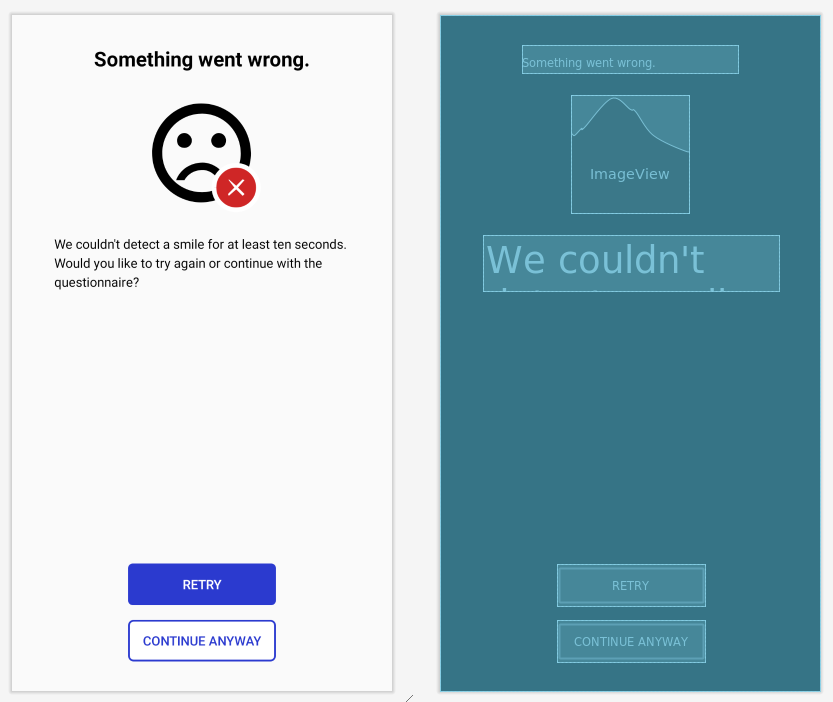
\includegraphics[width=\linewidth]{figures/user_interface.png}
  \caption{Example of a UI fragment designed in Android Studio's Layout Editor. A rendered screen is shown on the left, while its blueprint is depicted on the right.}
  \label{fig:user_interface}
\end{figure}

In terms of design, Android apps are generally expected to conform to Material Design, a set of guidelines defined by Google to help ensure both visual and practical consistency. As such, the user interface of the soHappy app is designed with Material Design in mind \cite{material_design}, incorporating principles such as animation or design based on the real world.
